\documentclass[10pt,aspectratio=169]{beamer}

\usetheme{AICL}

\usepackage{amsmath, amssymb}
\usepackage{booktabs}
\usepackage{graphicx}

\title{IFC Power Control via RIBBO}
\subtitle{Appendix / Backup Slides --- June 2026}
\author{Myoungjin Oh}
\date{\today}

\newenvironment{tightitemize}{%
    \begin{itemize}
        \setlength{\itemsep}{2pt}
        \setlength{\parskip}{0pt}
}{%
    \end{itemize}
}

\begin{document}

\begin{frame}[plain]
    \titlepage
\end{frame}

% ----------------------------------------------------------------
\section{Synthesis}
\begin{frame}{Synthesis --- RIBBO vs Dimension (SE \& EE)}
    \small
    \begin{columns}[T,onlytextwidth]
        \begin{column}{0.40\textwidth}
            \textbf{The whole story in one view} (3BA recipe, gap to optimum)
            \begin{tightitemize}
                \item EE $D{=}3$: smallest gap (3.5\%); gap grows with $D$ for both
                \item \textbf{RIBBO's gap far below Random at EE $D{=}10$} (48.7 pts smaller)
                \item SE: RIBBO and Random gaps stay close (on/off solutions are simple)
                \item $D{=}20$: large gap ($\sim$70\%) --- recipe/data limit (budget doesn't fix it)
            \end{tightitemize}
            \par\vspace{0.3em}
            {\scriptsize ``why RIBBO'' $=$ green solid-vs-dotted gap (EE, mid/high $D$).}
        \end{column}
        \begin{column}{0.58\textwidth}
            \centering
            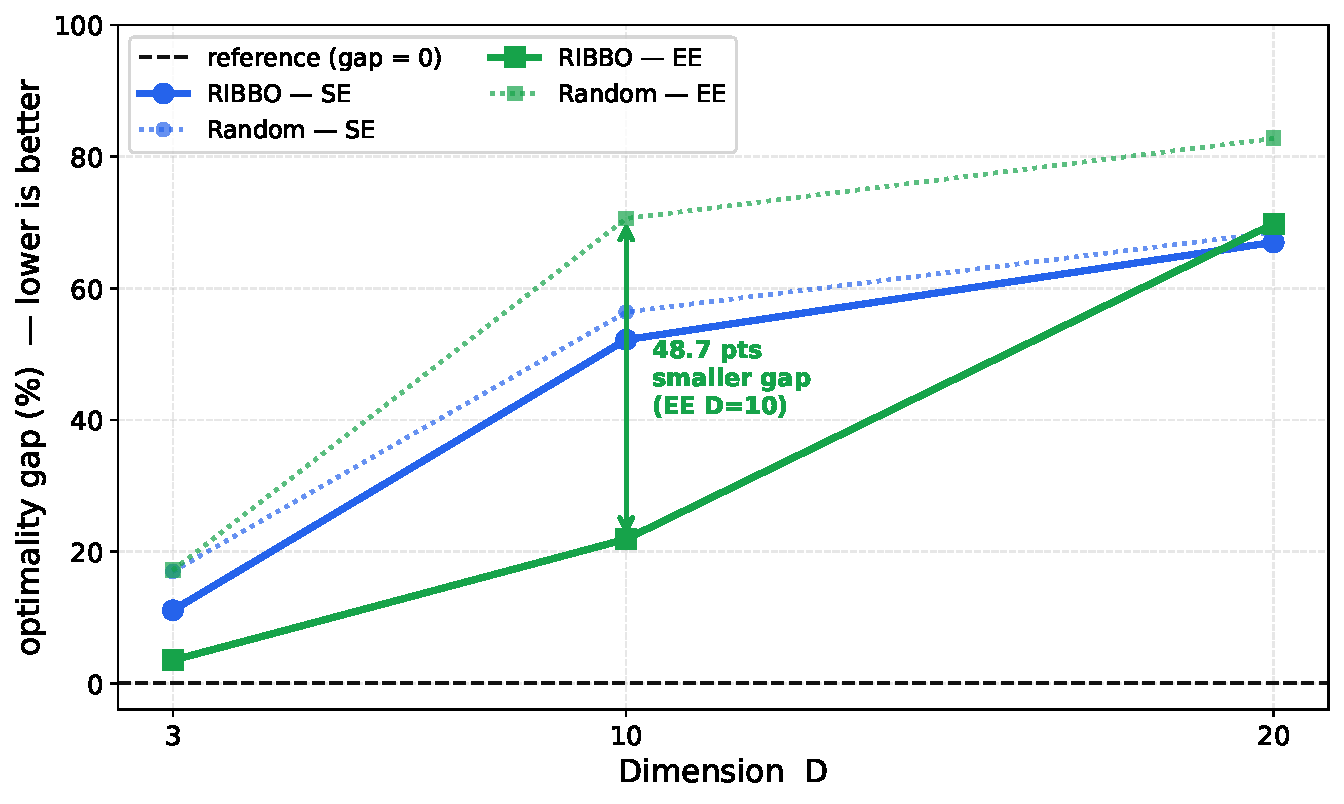
\includegraphics[width=\linewidth,height=0.70\textheight,keepaspectratio]{fig_synthesis.pdf}
        \end{column}
    \end{columns}
\end{frame}

% ----------------------------------------------------------------
\section{Sample efficiency}
\begin{frame}{Backup --- Sample Efficiency}
    \small
    \begin{columns}[T,onlytextwidth]
        \begin{column}{0.40\textwidth}
            \textbf{How fast does each method shrink the gap to optimum?}
            \begin{tightitemize}
                \item RIBBO inference is cheap $\Rightarrow$ ``just run longer''
                \item \textbf{SE $D{=}10$:} RIBBO gets the gap below 20\% by $\sim$815 evals; Random stays above 50\% within the budget ($\sim$53\%)
                \item \textbf{EE $D{=}10$:} RIBBO gets the gap below 30\% by $\sim$82 evals; Random stays above 50\% ($\sim$71\%)
                \item \textbf{SE $D{=}3$:} RIBBO $9\times$ faster to a 30\% gap; reaches a 10\% gap where Random stalls at 13\%
            \end{tightitemize}
        \end{column}
        \begin{column}{0.58\textwidth}
            \centering
            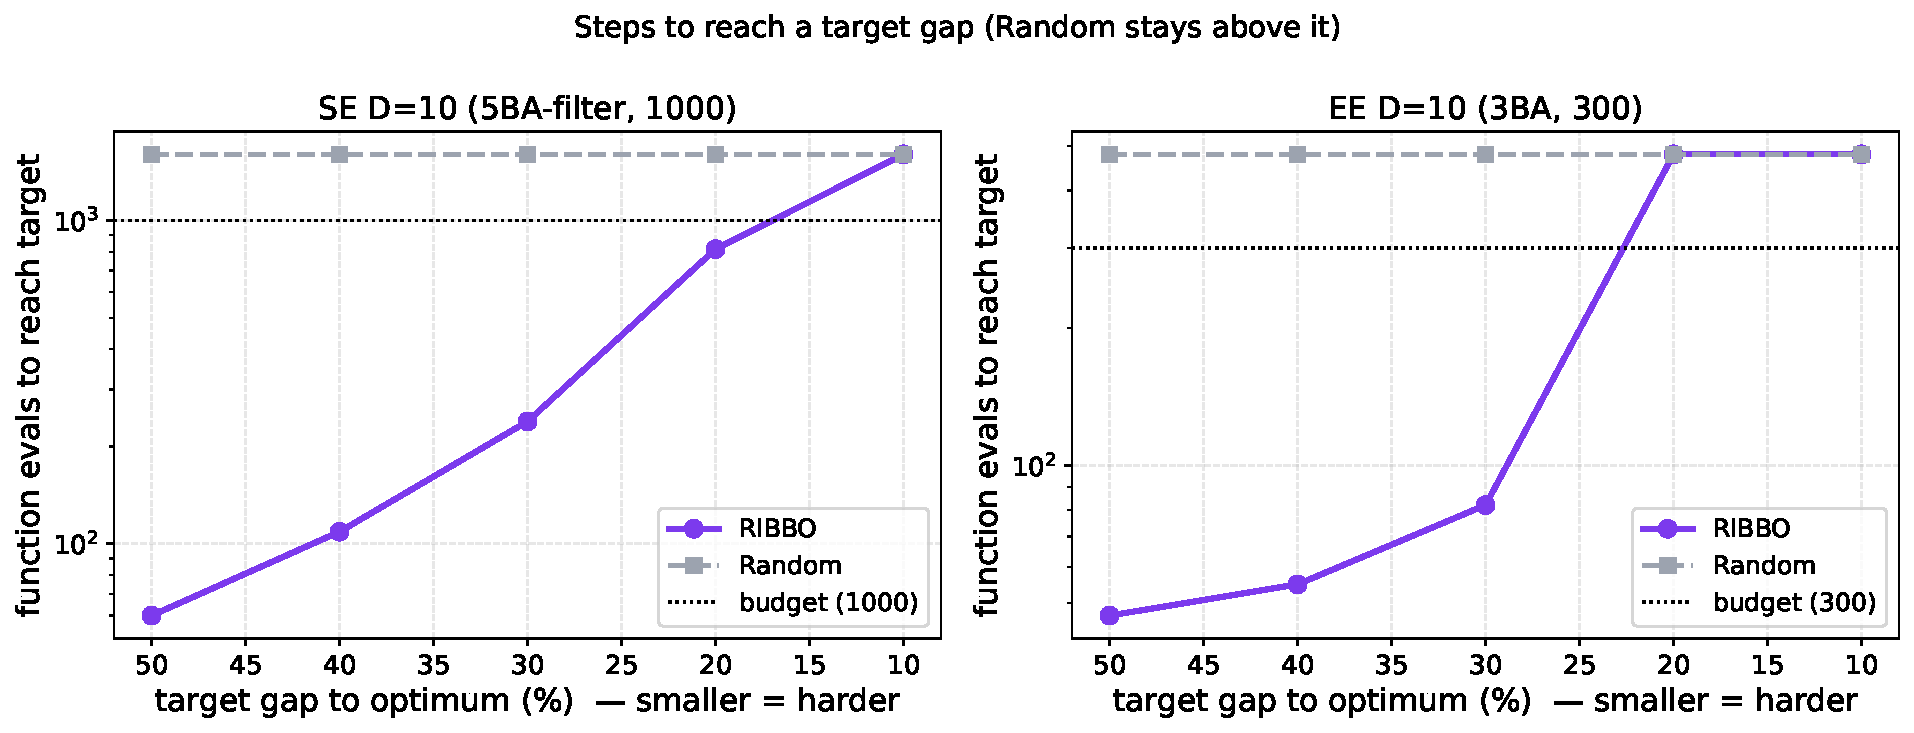
\includegraphics[width=\linewidth,height=0.68\textheight,keepaspectratio]{fig_sample_eff.pdf}
            \par{\scriptsize Random pinned above the budget line $=$ does not reach that target within the budget.}
        \end{column}
    \end{columns}
\end{frame}

% ----------------------------------------------------------------
\section{Per-channel}
\begin{frame}{Backup --- Per-Channel Statistics (beyond the mean)}
    \small
    \begin{columns}[T,onlytextwidth]
        \begin{column}{0.42\textwidth}
            \textbf{Win-rate \& distribution over channels} (300-step horizon)
            \par\vspace{0.3em}
            \scriptsize
            \begin{tabular}{lrrr}
                \toprule
                Case                & win-rate & R med gap & Rnd med gap \\
                \midrule
                SE $D{=}3$          & 73.6\%   & 3.7    & 15.4      \\
                SE $D{=}10$ (5BA)   & \textbf{100\%} & 27.7 & 57.2 \\
                EE $D{=}3$          & 88.5\%   & 2.0    & 15.4      \\
                EE $D{=}10$         & \textbf{100\%} & 20.6 & 70.9 \\
                SE $D{=}20$ (4BA)   & 99.5\%   & 58.5    & 68.1      \\
                \bottomrule
            \end{tabular}
            \par\vspace{0.4em}
            \begin{tightitemize}
                \item win-rate $=$ \% of channels where RIBBO's gap is smaller than Random's
                \item At $D{=}10$ RIBBO has a smaller gap than Random on \textbf{every} channel (SE and EE)
            \end{tightitemize}
        \end{column}
        \begin{column}{0.56\textwidth}
            \centering
            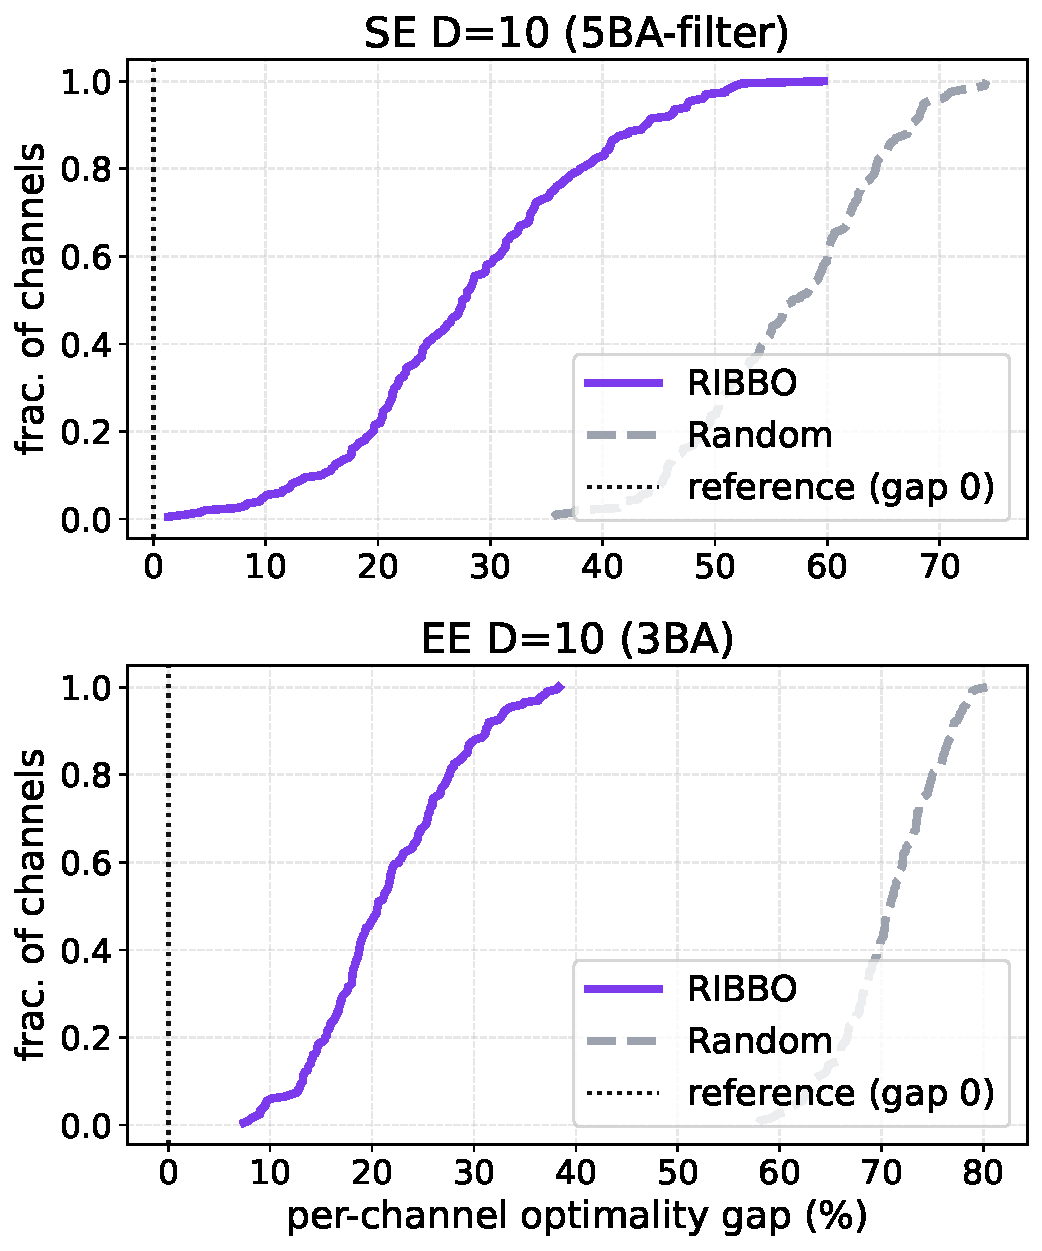
\includegraphics[width=\linewidth,height=0.68\textheight,keepaspectratio]{fig_per_channel.pdf}
            \par{\scriptsize CDF shifted left $=$ more channels with small gap (closer to optimum).}
        \end{column}
    \end{columns}
\end{frame}

% ----------------------------------------------------------------
\section{WMMSE}
\begin{frame}{Backup --- WMMSE Baseline Validation (SE $D{=}3$)}
    \small
    \begin{columns}[T,onlytextwidth]
        \begin{column}{0.42\textwidth}
            \textbf{Our WMMSE is the true optimum}
            \begin{tightitemize}
                \item Shi 2011 box-constrained WMMSE, 10 restarts
                \item Matches brute-force grid: gap $0/10$ channels
                \item Our value 2.864 nats vs Lee 2.50 (channel-distribution / setup difference; we use the \emph{same} channels for a fair RIBBO-vs-WMMSE comparison)
                \item RIBBO 3BA gets within \textbf{11.1\% gap} of WMMSE
            \end{tightitemize}
        \end{column}
        \begin{column}{0.56\textwidth}
            \centering
            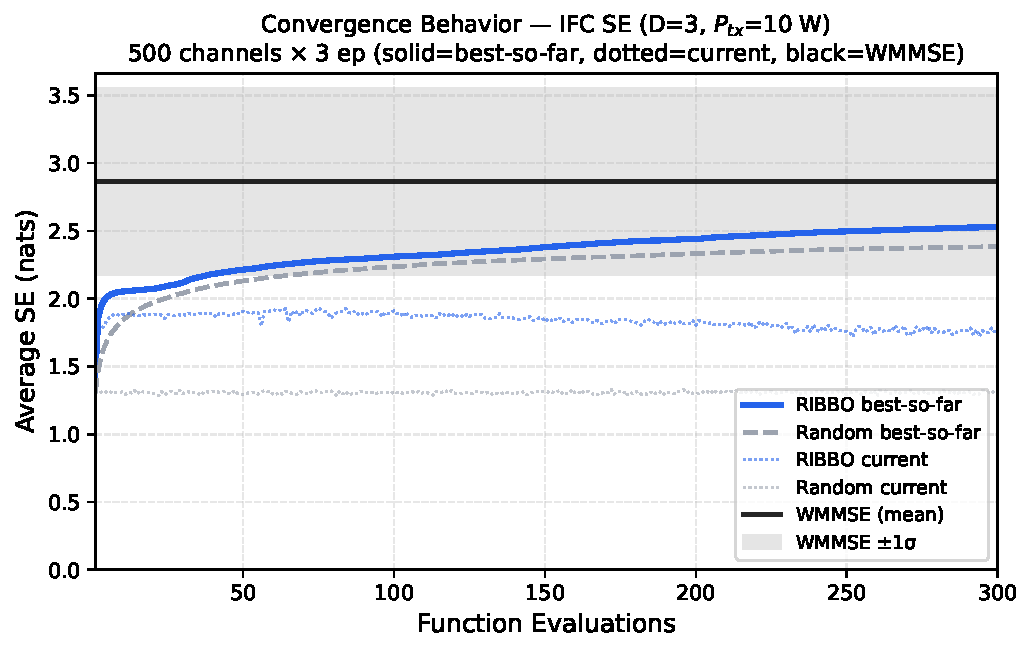
\includegraphics[width=\linewidth,height=0.68\textheight,keepaspectratio]{fig_wmmse_d3.pdf}
        \end{column}
    \end{columns}
\end{frame}

% ----------------------------------------------------------------
\section{EE pool}
\begin{frame}{Backup --- BA-pool Curation Is Problem-Dependent (EE)}
    \small
    \begin{columns}[T,onlytextwidth]
        \begin{column}{0.42\textwidth}
            \textbf{For EE, dropping Random \emph{lowers performance}}
            \par\vspace{0.3em}
            \scriptsize
            \begin{tabular}{lrr}
                \toprule
                EE $D{=}10$ model        & RIBBO gap & Random gap \\
                \midrule
                3BA (incl.\ Random)      & \textbf{21.9} & 70.6 \\
                4BA-filter (no Random)   & 30.3          & 70.6 \\
                \bottomrule
            \end{tabular}
            \par\vspace{0.4em}
            \begin{tightitemize}
                \item Opposite of SE high-$D$ (where curation \emph{shrinks} the gap 23.6 pts)
                \item EE optimum is interior/low-power; Random's broad low-power coverage is genuinely useful
                \item $\Rightarrow$ don't reuse the SE recipe blindly for EE
            \end{tightitemize}
        \end{column}
        \begin{column}{0.56\textwidth}
            \centering
            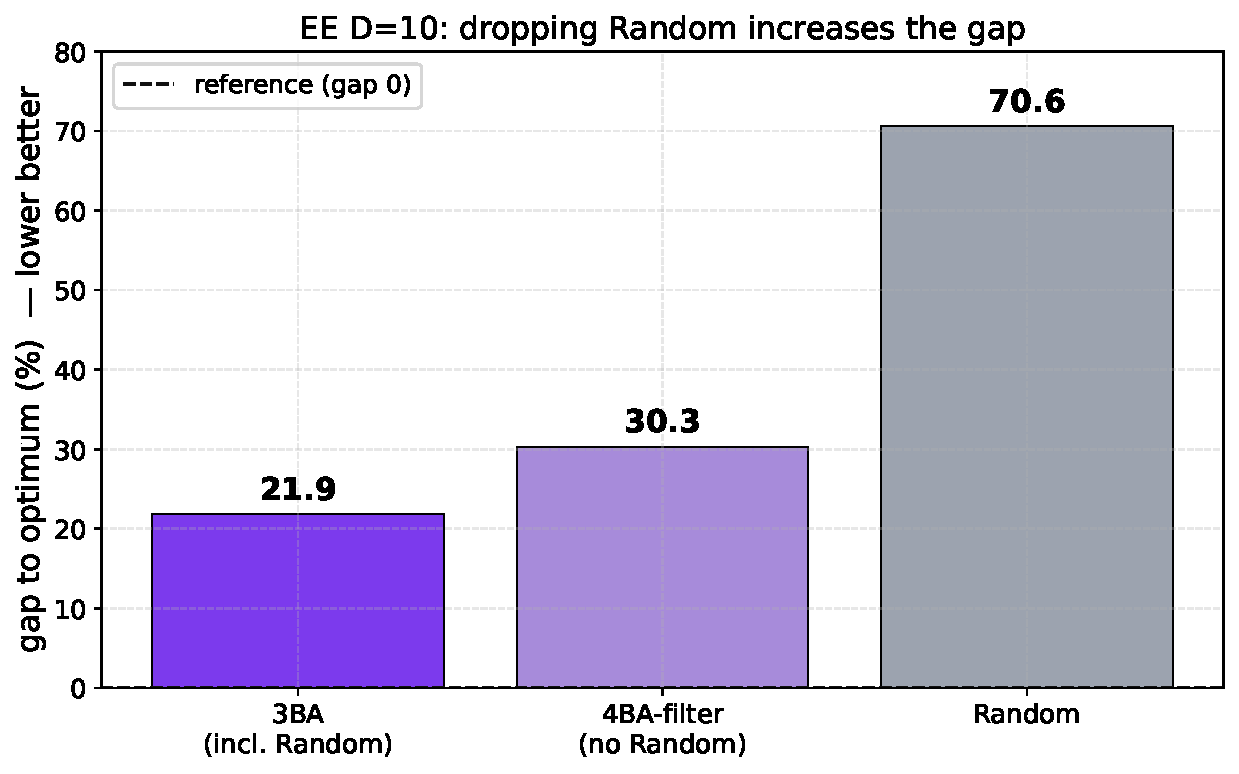
\includegraphics[width=\linewidth,height=0.68\textheight,keepaspectratio]{fig_ee_pool.pdf}
        \end{column}
    \end{columns}
\end{frame}

% ----------------------------------------------------------------
\section{Budget}
\begin{frame}{Backup --- Evaluation Budget Extension}
    \small
    \begin{columns}[T,onlytextwidth]
        \begin{column}{0.40\textwidth}
            \textbf{Run longer $\Rightarrow$ smaller gap} (inference is cheap)
            \begin{tightitemize}
                \item SE $D{=}3$ 3BA: gap $13.0 \to \textbf{8.3}$ ($-4.8$ pts) at 1000 steps
                \item SE $D{=}10$ 5BA-filter: gap $27.1 \to \textbf{19.0}$ ($-8.1$ pts)
                \item Higher dimension $\Rightarrow$ larger budget gain
            \end{tightitemize}
        \end{column}
        \begin{column}{0.58\textwidth}
            \centering
            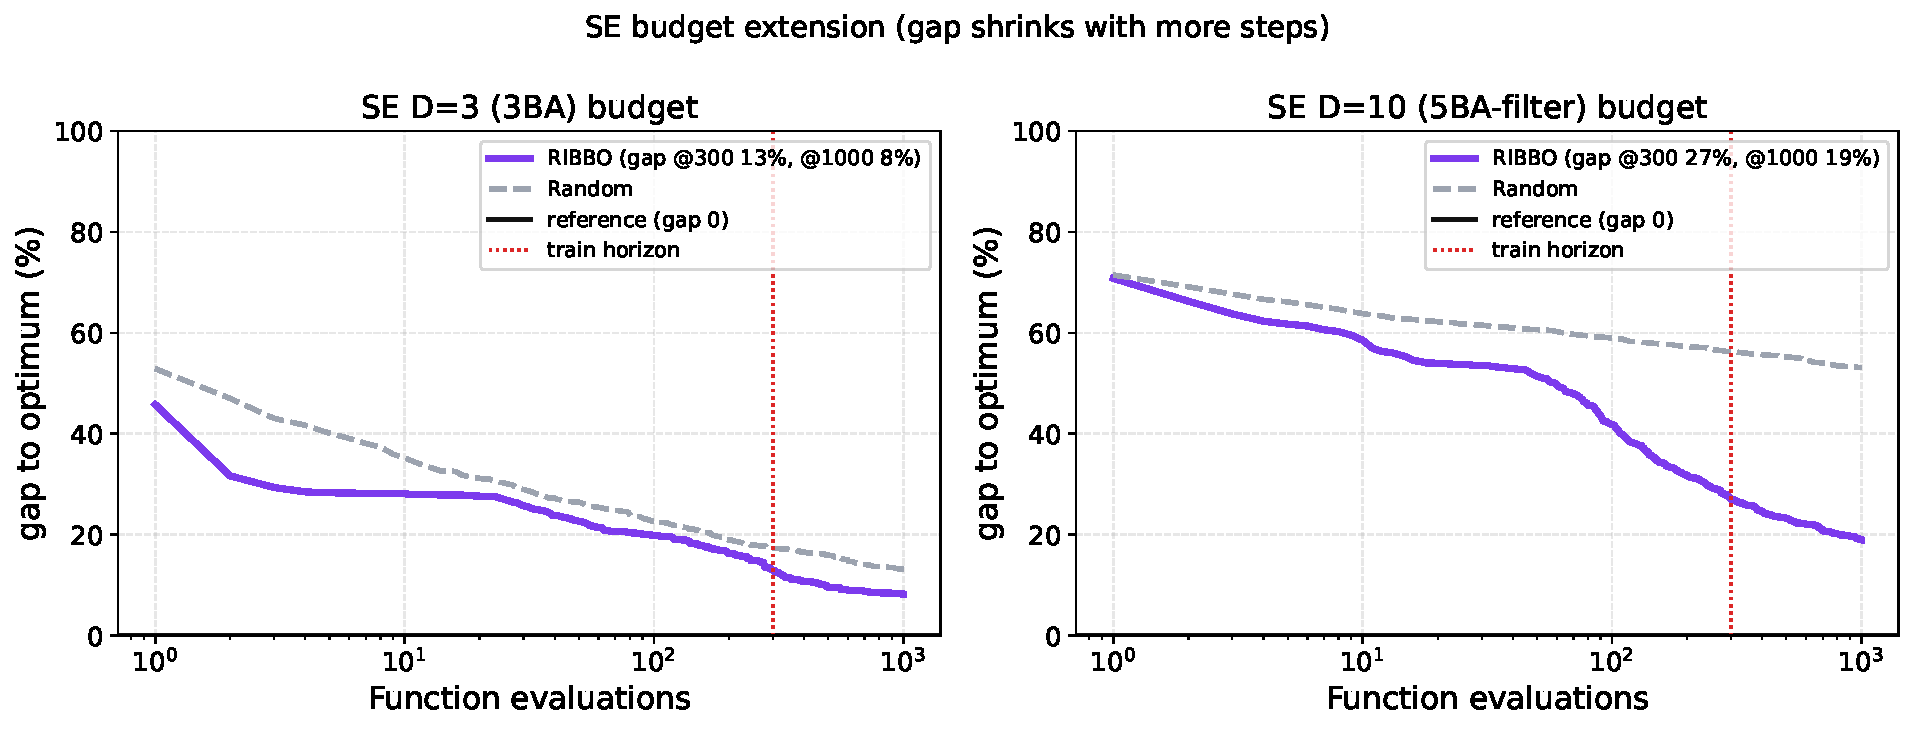
\includegraphics[width=\linewidth,height=0.68\textheight,keepaspectratio]{fig_budget.pdf}
        \end{column}
    \end{columns}
\end{frame}

% ----------------------------------------------------------------
\section{All numbers}
\begin{frame}{Backup --- Full Results Table}
    \small
    \centering
    \begin{tabular}{llrrr}
        \toprule
        Objective & Setting & RIBBO gap & Random gap & RIBBO saves \\
        \midrule
        SE & $D{=}3$  (3BA)            & 11.1 & 17.0 & $5.9$  \\
        SE & $D{=}10$ (3BA)            & 52.2 & 56.4 & $4.2$  \\
        SE & $D{=}10$ (5BA-filter)     & \textbf{28.6} & 56.4 & $27.8$ \\
        SE & $D{=}20$ (3BA)            & 67.0 & 68.5 & $1.5$  \\
        SE & $D{=}20$ (4BA-filter)     & \textbf{58.1} & 68.5 & $10.4$ \\
        \midrule
        EE & $D{=}3$  (3BA)            & 3.5 & 17.2 & $13.7$ \\
        EE & $D{=}10$ (3BA)            & \textbf{21.9} & 70.6 & $\mathbf{48.7}$ \\
        EE & $D{=}10$ (4BA-filter)     & 30.3 & 70.6 & $40.3$ \\
        \bottomrule
    \end{tabular}

    \vspace{0.6em}
    {\footnotesize gap to optimum (\%), lower better. Budget (1000 steps): SE $D{=}3$ gap $\to 8.3$, SE $D{=}10$ gap $\to 19.0$. \quad
    Win-rate $D{=}10$: SE \& EE both 100\% of channels.}
\end{frame}

% ----------------------------------------------------------------
\section{EE D=20}
\begin{frame}{Backup --- EE at $D{=}20$ \hfill {\small\textit{(new, trained overnight)}}}
    \small
    \begin{columns}[T,onlytextwidth]
        \begin{column}{0.42\textwidth}
            \textbf{The EE advantage persists at $D{=}20$}
            \par\vspace{0.3em}
            \scriptsize
            \begin{tabular}{lrr}
                \toprule
                EE $D{=}20$ (3BA) & gap to opt & 95\% CI \\
                \midrule
                RIBBO   & \textbf{69.8} & $\pm0.8$ \\
                Random  & 82.8          & $\pm0.3$ \\
                \bottomrule
            \end{tabular}
            \par\vspace{0.4em}
            \begin{tightitemize}
                \item RIBBO's gap is \textbf{13.0 pts smaller}, \textbf{100\%} win-rate
                \item Bigger lead than SE $D{=}20$ (13.0 vs 10.4 pts smaller) --- the interior EE optimum keeps RIBBO valuable
                \item Gap grows with $D$ (fixed 3BA recipe). \textbf{Budget does \emph{not} shrink it} (next slide) --- a data/recipe limit, not budget
            \end{tightitemize}
        \end{column}
        \begin{column}{0.56\textwidth}
            \centering
            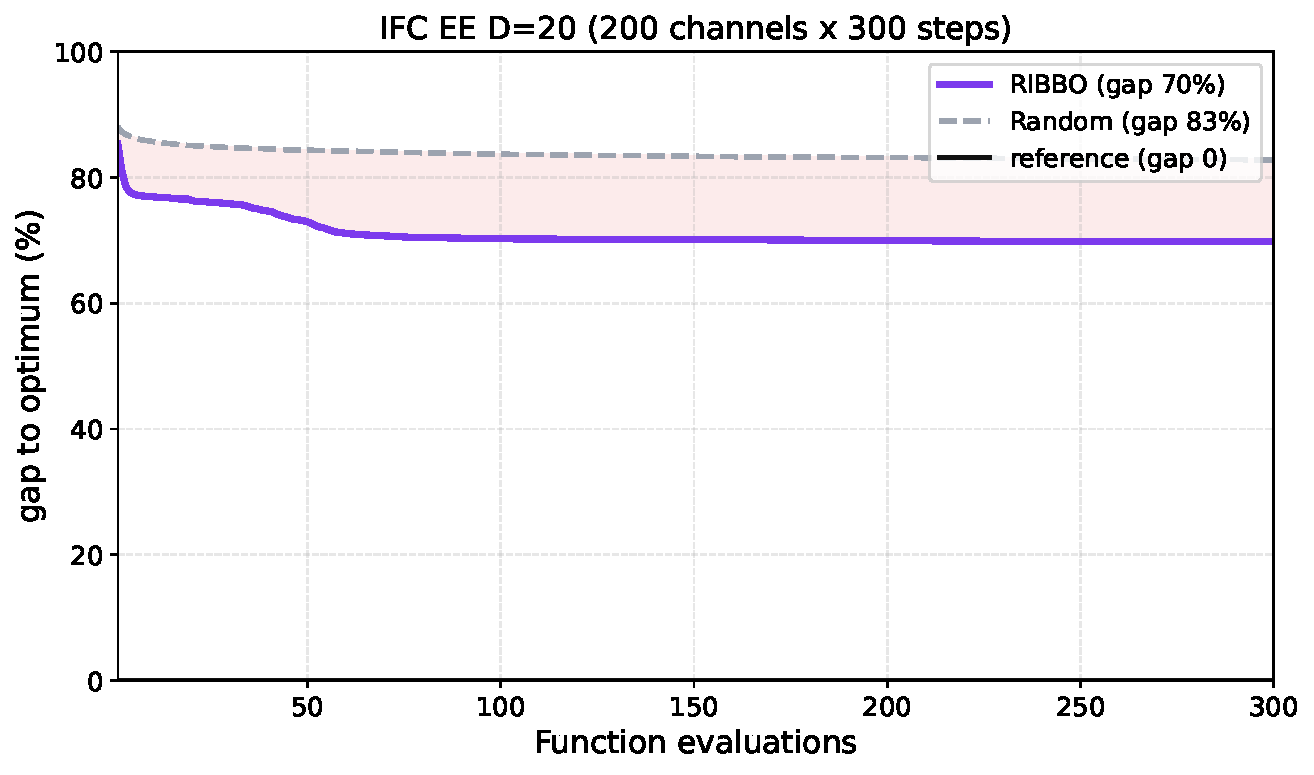
\includegraphics[width=\linewidth,height=0.66\textheight,keepaspectratio]{fig_ee_d20.pdf}
        \end{column}
    \end{columns}
\end{frame}

% ----------------------------------------------------------------
\section{EE D=20 budget}
\begin{frame}{Backup --- EE $D{=}20$: Budget Does \emph{Not} Recover It}
    \small
    \begin{columns}[T,onlytextwidth]
        \begin{column}{0.42\textwidth}
            \textbf{Running longer (300 $\to$ 1000 steps) gives almost no gain here}
            \begin{tightitemize}
                \item RIBBO gap @300 $=69.9\%$ $\to$ @1000 $=69.7\%$ (\textbf{$-0.2$ pts})
                \item Contrast: SE budget shrank the gap 8.1 pts (D=10), 4.8 (D=3)
                \item RIBBO's gap plateaus high $\Rightarrow$ the model has saturated, not under-budgeted
            \end{tightitemize}
            \par\vspace{0.4em}
            \textbf{Refines the ``recovery levers'' claim:} budget helps only while the model is still improving (SE). EE $D{=}20$'s gap is a \textbf{data-capacity limit} --- it needs more channels/data, not more steps.
        \end{column}
        \begin{column}{0.56\textwidth}
            \centering
            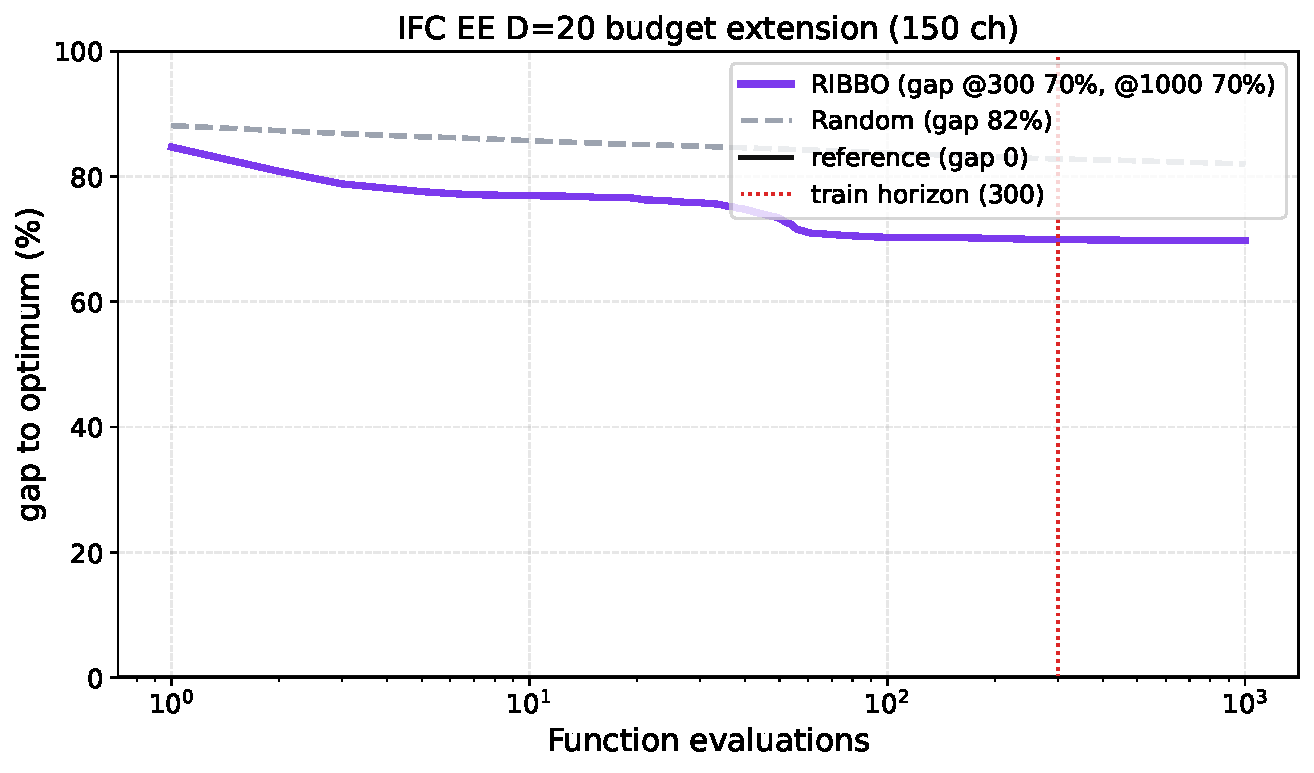
\includegraphics[width=\linewidth,height=0.66\textheight,keepaspectratio]{fig_ee_d20_budget.pdf}
            \par{\scriptsize Flat past $\sim$50 evals; train-horizon line at 300 makes no difference.}
        \end{column}
    \end{columns}
\end{frame}

% ----------------------------------------------------------------
\section{Hybrid}
\begin{frame}{Backup --- Hybrid: RIBBO $+$ Local Polish}
    \small
    \begin{columns}[T,onlytextwidth]
        \begin{column}{0.42\textwidth}
            \textbf{A cheap local search reaches $\sim$optimum from \emph{either} starting point}
            \par\vspace{0.3em}
            \scriptsize
            \begin{tabular}{lrr}
                \toprule
                gap to optimum   & EE $D{=}10$ & SE $D{=}20$ \\
                \midrule
                RIBBO             & 20.6        & 58.9        \\
                RIBBO $+$ polish  & \textbf{0.2} & \textbf{3.4} \\
                Random            & 70.6        & 68.5        \\
                Random $+$ polish & 0.7         & 2.6         \\
                \bottomrule
            \end{tabular}
            \par\vspace{0.4em}
            \begin{tightitemize}
                \item Polish dominates; the init barely matters (RIBBO $\approx$ Random after polish)
                \item $\Rightarrow$ with the channel model/gradients a local search reaches the optimum (as WMMSE/FP do); RIBBO's value is the \textbf{no-model} case
            \end{tightitemize}
        \end{column}
        \begin{column}{0.56\textwidth}
            \centering
            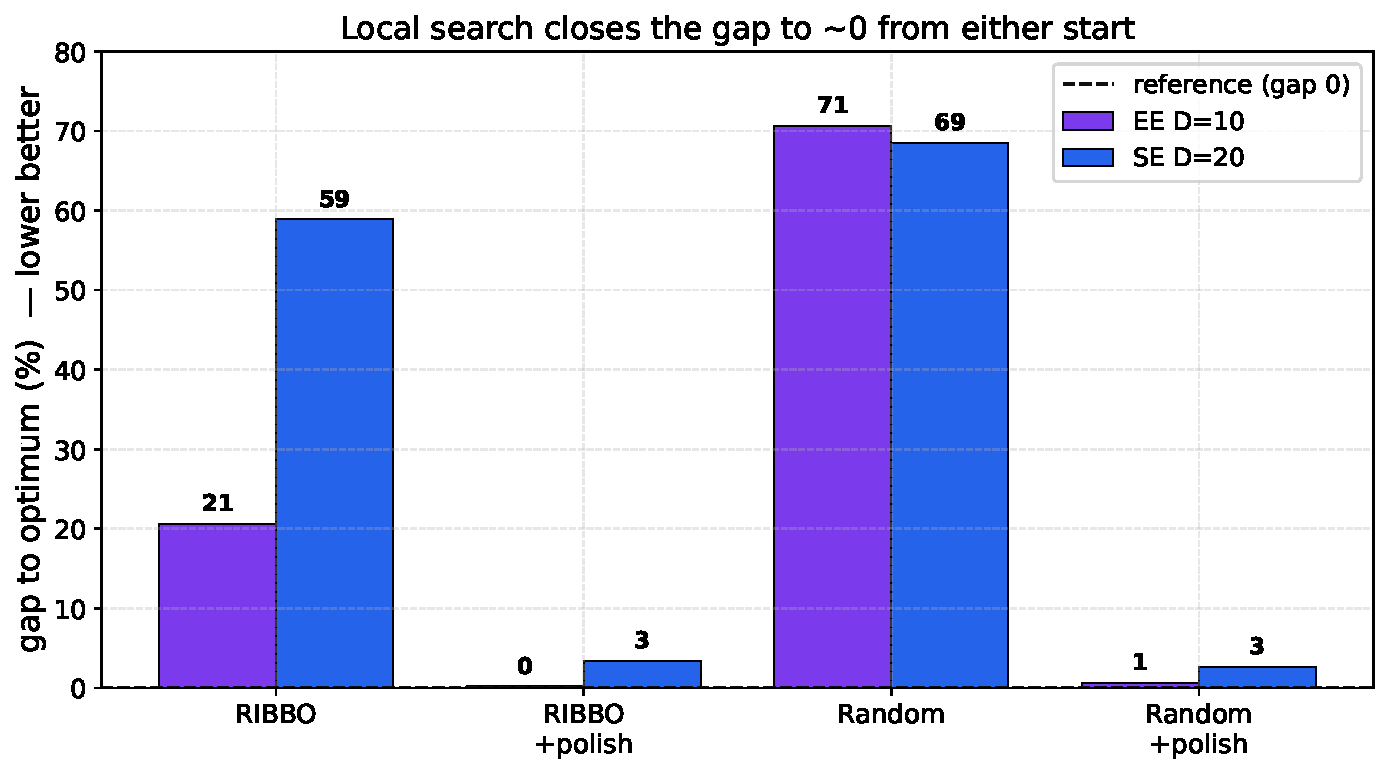
\includegraphics[width=\linewidth,height=0.66\textheight,keepaspectratio]{fig_hybrid.pdf}
        \end{column}
    \end{columns}
\end{frame}

% ----------------------------------------------------------------
\section{Confidence}
\begin{frame}{Backup --- 95\% Confidence Intervals (robustness)}
    \small
    \centering
    \begin{tabular}{llrrr}
        \toprule
        Obj. & Setting & RIBBO gap ($\pm$CI) & Random gap ($\pm$CI) & win-rate \\
        \midrule
        SE & $D{=}3$ (3BA)         & $10.7 \pm 1.3$ & $17.8 \pm 1.0$ & 73.6\% \\
        SE & $D{=}10$ (5BA-filter) & $28.4 \pm 1.5$ & $56.7 \pm 1.2$ & \textbf{100\%} \\
        SE & $D{=}20$ (4BA-filter) & $58.0 \pm 1.0$ & $68.5 \pm 0.7$ & 99.5\% \\
        EE & $D{=}3$ (3BA)         & $3.2 \pm 0.5$ & $17.6 \pm 1.7$ & 88.5\% \\
        EE & $D{=}10$ (3BA)        & $21.5 \pm 1.0$ & $70.6 \pm 0.7$ & \textbf{100\%} \\
        EE & $D{=}20$ (3BA)        & $69.8 \pm 0.8$ & $82.8 \pm 0.3$ & \textbf{100\%} \\
        \bottomrule
    \end{tabular}

    \vspace{0.6em}
    {\footnotesize gap to optimum (\%), lower better. $\pm$ is 95\% CI ($1.96\,\mathrm{sd}/\sqrt{n}$), $n{=}200$. \;
    500-channel re-eval confirms: EE $D{=}10$ $20.7\pm0.7$, SE $D{=}20$ $58.6\pm0.6$. \;
    Intervals are narrow $\Rightarrow$ not sampling artifacts.}
\end{frame}

\end{document}
